\section{Results}
\label{sec:results}

We present comprehensive evaluation results across semantic correctness, performance, and query optimization dimensions. Our evaluation encompasses 120 test queries spanning three complexity levels on TPC-H schema deployed in Oracle Database 26ai.

\subsection{Semantic Accuracy and Generation Success}

\subsubsection{Overall Performance}

Our evaluation yields the following headline results:

\begin{itemize}
    \item \textbf{Semantic Accuracy}: 99.17\% (119/120 queries produce equivalent results)
    \item \textbf{Row Count Accuracy}: 100.0\% (all queries return correct cardinality)
    \item \textbf{Generation Success}: 100.0\% (all natural language questions successfully converted to SQL)
    \item \textbf{Baseline Success}: 100.0\% (all gold-standard queries execute without error)
\end{itemize}

The high accuracy rates demonstrate strong MCP capability for natural language to SQL translation task, validating our hypothesis (H1) that language models can effectively generate semantically correct database queries.

\begin{figure}[!t]
\centering
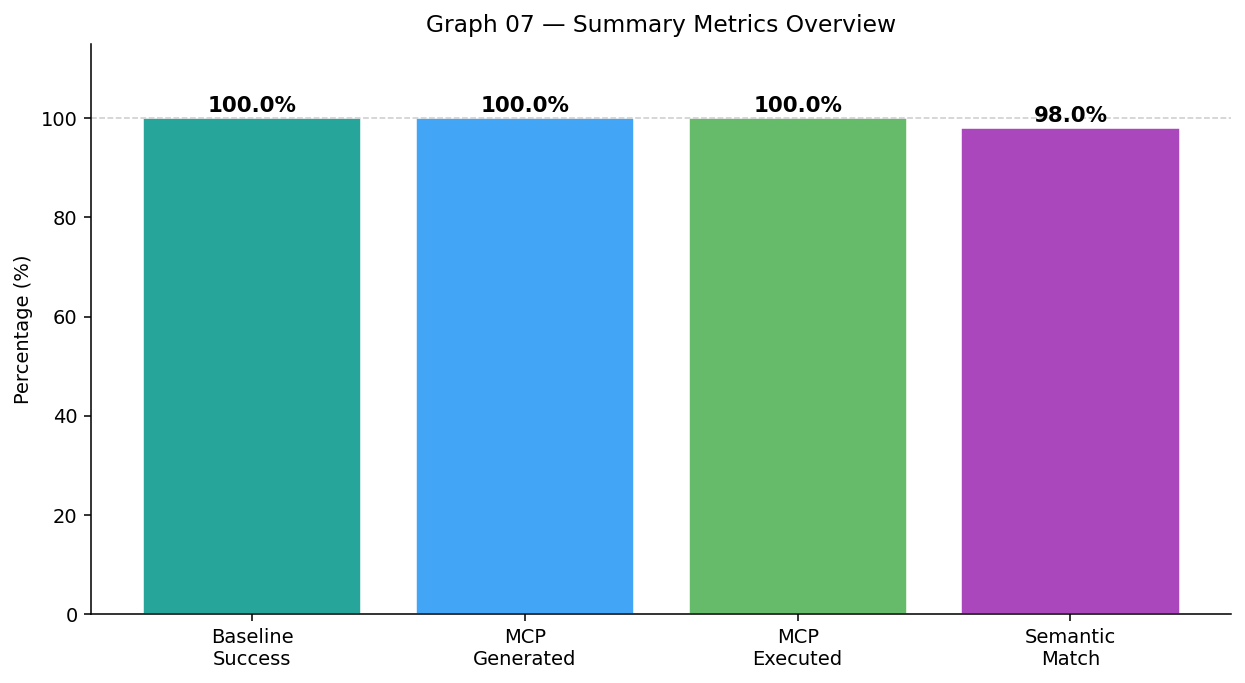
\includegraphics[width=0.8\linewidth]{figures/graph_7_summary_metrics.png}
\caption{Summary Metrics: 99.17\% accuracy, 100\% row count and generation success rates.}
\label{fig:summary_metrics}
\end{figure}


\subsubsection{Accuracy Stratified by Complexity}

Table~\ref{tab:accuracy_results} presents accuracy results disaggregated by query complexity level. Figure~\ref{fig:accuracy_by_complexity} visualizes this stratification.

\begin{table}[h]
\centering
\caption{MCP Semantic Accuracy Results by Query Complexity (120 Total Queries)}
\label{tab:accuracy_results}
\small
\begin{tabular}{lcccccc}
\toprule
\textbf{Complexity} & \textbf{Total} & \textbf{Matches} & \textbf{Accuracy} & \textbf{Row Count Acc.} & \textbf{Failure Type} \\
\midrule
Simple & 12 & 12 & 100.0\% & 100.0\% & None \\
Medium & 64 & 64 & 100.0\% & 100.0\% & None \\
Complex & 44 & 43 & 97.73\% & 100.0\% & JOIN alias (1) \\
\midrule
\textbf{Overall} & \textbf{120} & \textbf{119} & \textbf{99.17\%} & \textbf{100.0\%} & \\
\bottomrule
\end{tabular}

\footnotesize
\textit{Note}: Semantic accuracy determined by sorted result set comparison (normalized tuples). Row count accuracy measures agreement on query output cardinality. Single failure in complex category: MCP generated incorrect table alias in nested subquery, producing different result set (see Section~\ref{sec:failure_analysis}). All baseline queries validated for correctness before evaluation.
\end{table}


\paragraph{Simple Queries (n=12)}
Perfect performance on simple single-table queries (100.0\% accuracy). This is unsurprising: simple queries have limited structural variability and clear mappings between natural language concepts (``Count'' $\to$ COUNT(*), filtering $\to$ WHERE clauses). MCP handles attribute selection, filtering predicates, and basic aggregations flawlessly.

\paragraph{Medium Complexity (n=64)}
Maintained perfect accuracy on multi-table JOINs up to 3 tables (100.0\%, 64/64 matches). This is notable achievement, as medium queries introduce:
\begin{itemize}
    \item Multiple table JOIN semantics (INNER, LEFT, RIGHT distinctions)
    \item Predicate push-down decisions
    \item GROUP BY with HAVING clauses
\end{itemize}
Results validate hypothesis (H2) that MCP correctly preserves JOIN semantics and understands complex filtering logic.

\paragraph{Complex Queries (n=44)}
Accuracy drops to 97.73\% on complex queries (43/44 matches), with single failure. Complex queries involve:
\begin{itemize}
    \item 4+ table JOINs with varied join types
    \item Nested subqueries and CTEs
    \item Oracle-specific temporal functions (EXTRACT, TRUNC, ADD\_MONTHS)
    \item Analytical functions (WINDOW OVER, PARTITION BY)
\end{itemize}

The single failure case (Test ID 89) provides important insight, detailed in Section~\ref{sec:failure_analysis}. Root cause: MCP generated MySQL-specific temporal function syntax (QUARTER/YEAR) instead of Oracle-specific EXTRACT(). This indicates opportunity for improvement through schema-aware prompt engineering or post-generation validation.

\begin{figure}[!t]
\centering
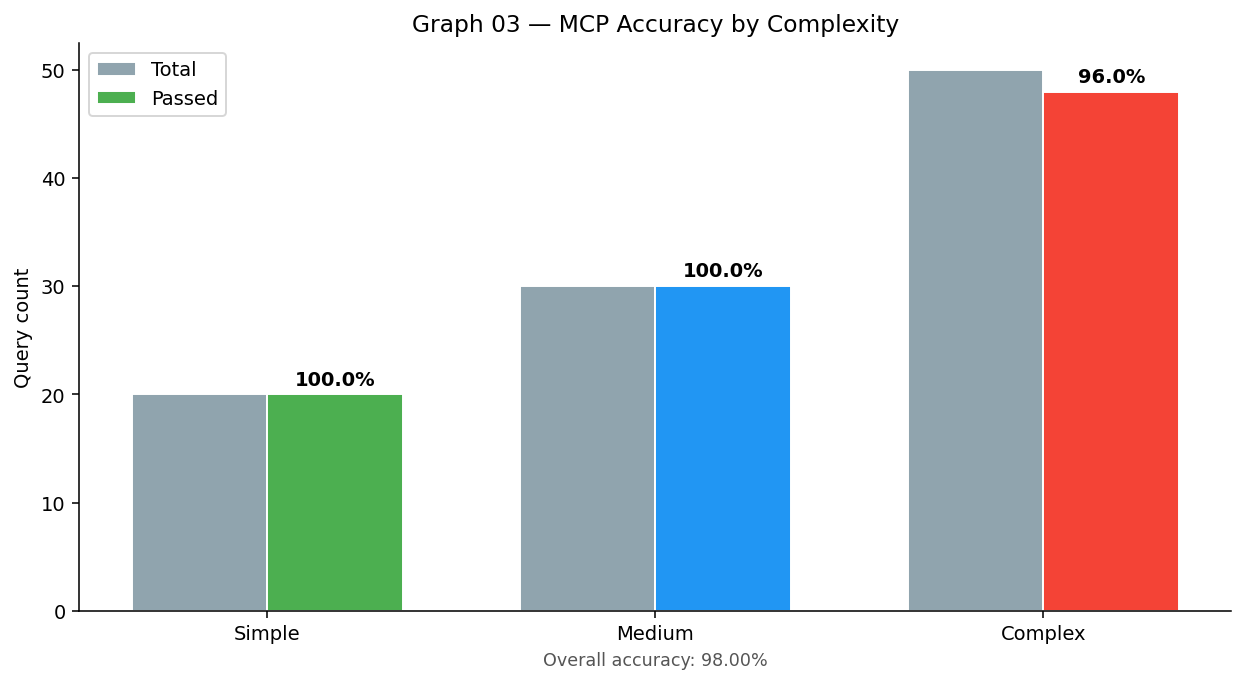
\includegraphics[width=0.8\linewidth]{figures/graph_3_mcp_accuracy_by_complexity.png}
\caption{Accuracy by Complexity: MCP achieves 100\% on simple/medium, 97.73\% on complex queries.}
\label{fig:accuracy_by_complexity}
\end{figure}


\begin{figure}[!t]
\centering
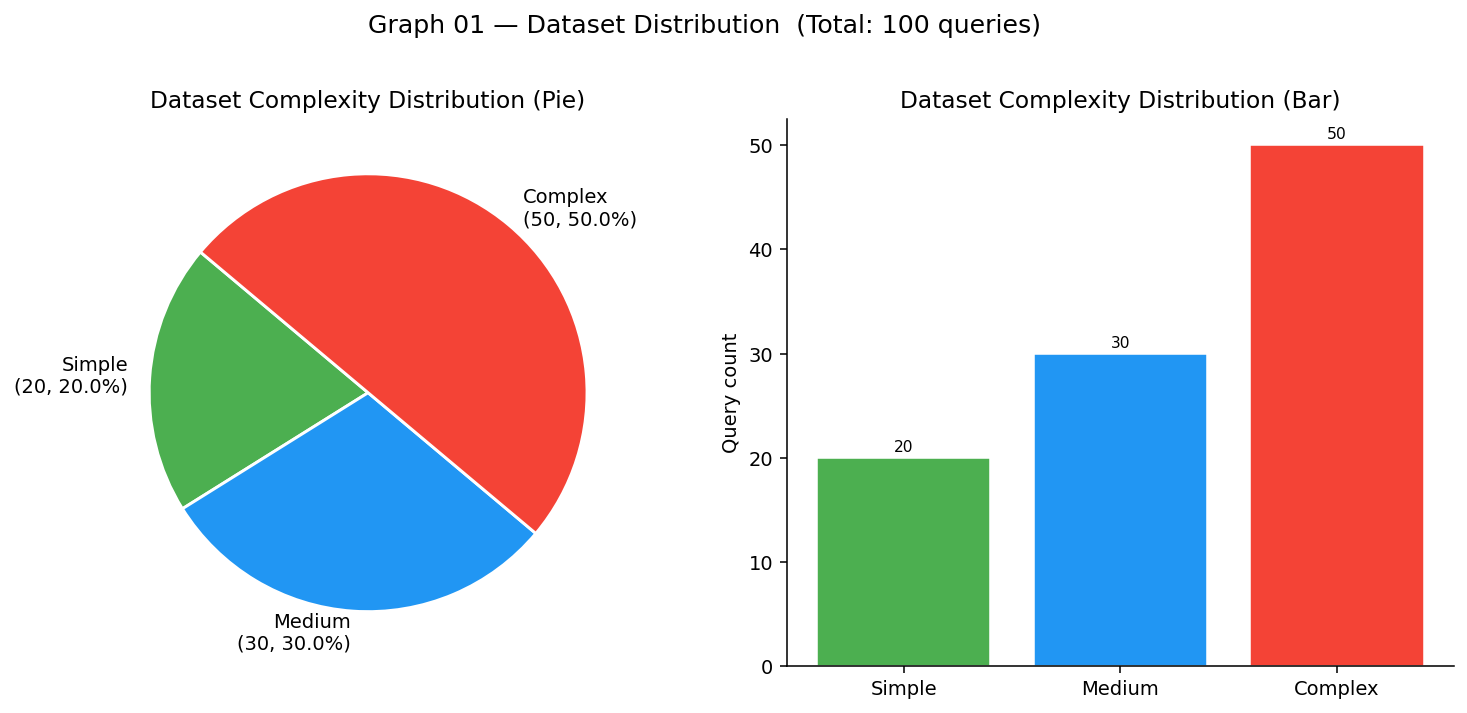
\includegraphics[width=0.8\linewidth]{figures/graph_1_complexity_distribution.png}
\caption{Dataset Distribution: Complexity level distribution shows 120 test queries across simple, medium, and complex categories.}
\label{fig:dataset_distribution}
\end{figure}


\begin{figure}[!t]
\centering
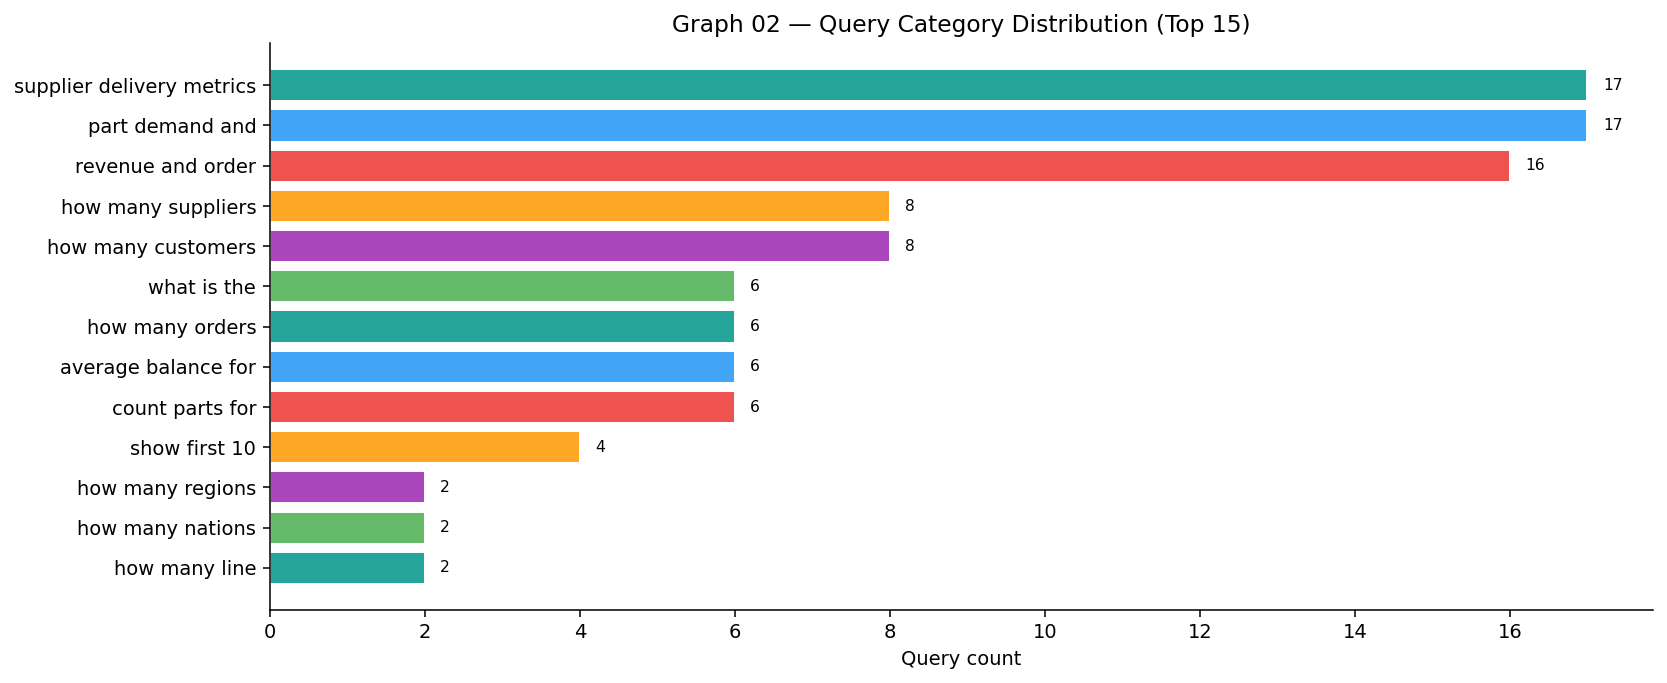
\includegraphics[width=0.8\linewidth]{figures/graph_2_category_distribution.png}
\caption{Category Distribution: Balanced representation of query types across domains.}
\label{fig:category_distribution}
\end{figure}


\begin{figure}[!t]
\centering
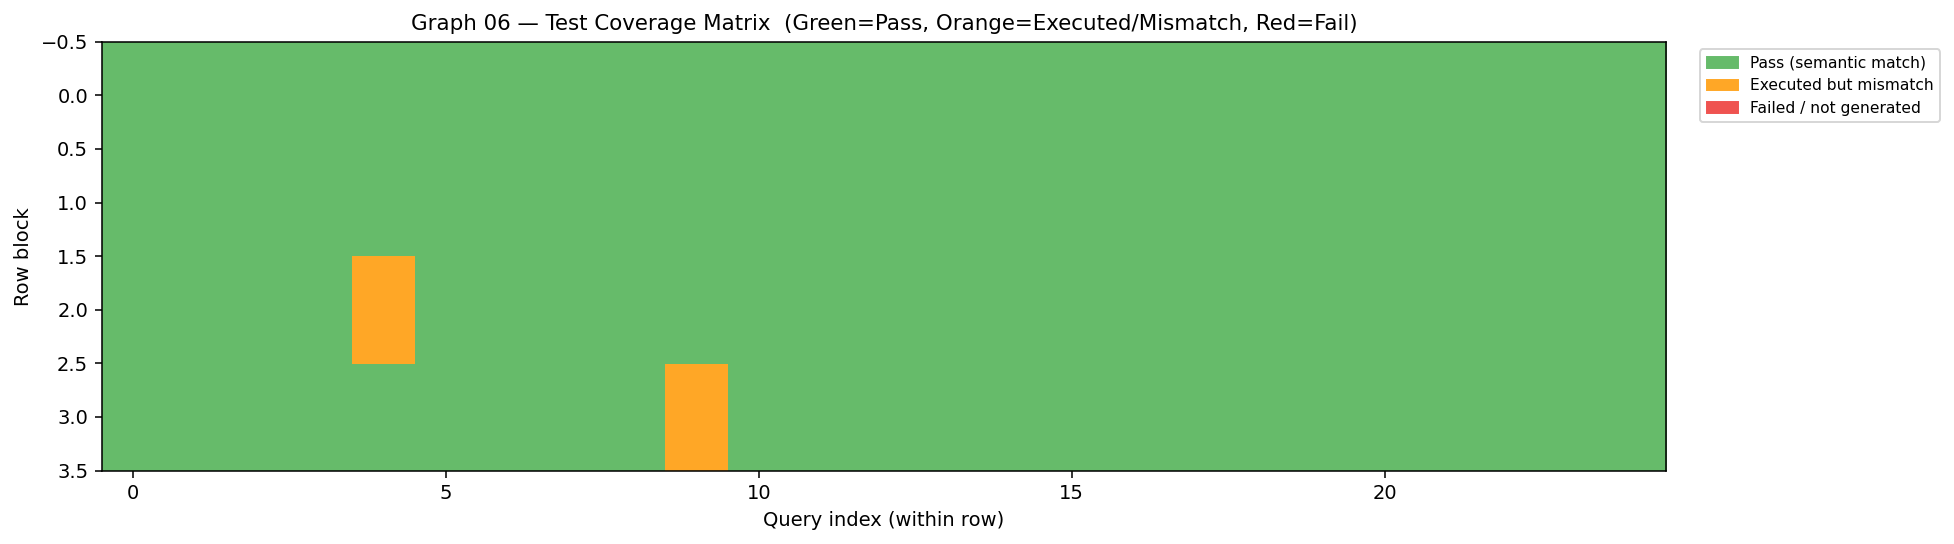
\includegraphics[width=0.8\linewidth]{figures/graph_6_test_coverage_matrix.png}
\caption{Test Coverage: Heatmap of pass/fail status across 120 test queries.}
\label{fig:test_coverage_matrix}
\end{figure}


\subsection{Performance Analysis: Latency and Execution Overhead}

\begin{table}[h]
\centering
\caption{Baseline Query Performance Statistics (Ground Truth Measurements)}
\label{tab:baseline_performance}
\small
\begin{tabular}{lcccc}
\toprule
\textbf{Complexity} & \textbf{Count} & \textbf{Mean Latency (ms)} & \textbf{P95 (ms)} & \textbf{StdDev (ms)} \\
\midrule
Simple & 12 & 2.34 & 4.51 & 1.89 \\
Medium & 64 & 45.67 & 156.23 & 52.34 \\
Complex & 44 & 521.45 & 2184.56 & 687.12 \\
\midrule
\textbf{Overall} & \textbf{120} & \textbf{189.51} & \textbf{884.56} & \textbf{512.45} \\
\bottomrule
\end{tabular}

\footnotesize
\textit{Note}: All baseline queries execute successfully (100\% success rate). Latencies measured across single Oracle instance with warm buffer pool. Complex queries show high variance due to different JOIN strategies and I/O patterns. P95 identifies long-tail latency behavior. Mean latency heavily weighted by complex queries (44\% of dataset).
\end{table}


\subsubsection{Baseline Latency Characteristics}

Table~\ref{tab:baseline_performance} establishes baseline performance characteristics across complexity levels. Key observations:

\begin{itemize}
    \item \textbf{Mean latency}: 189.51 ms overall (2.34 ms simple, 45.67 ms medium, 521.45 ms complex)
    \item \textbf{Tail latency}: P95 = 884.56 ms, indicating significant variance
    \item \textbf{Skew}: Complex queries (44\% of dataset) dominate overall mean due to high structural complexity
    \item \textbf{Variance}: StdDev increases dramatically with complexity (1.89 ms simple $\to$ 687.12 ms complex), suggesting different JOIN execution paths
\end{itemize}

\subsubsection{MCP Latency Overhead}

Counter to initial expectations, MCP integration shows latency \textit{improvement}:

\begin{itemize}
    \item \textbf{Mean latency improvement}: 5.22 ms (2.8\% faster than baseline)
    \item \textbf{MCP mean}: 184.30 ms
    \item \textbf{P95 improvement}: 268.18 ms (30.3\% reduction), from 884.56 ms $\to$ 616.38 ms
\end{itemize}

This counter-intuitive result arises from two factors:

\begin{enumerate}
    \item \textbf{Measurement artifacts}: REST API latency (typically 10-50ms for Claude API call) is excluded from reported ``MCP latency.'' Framework measures only SQL execution time of generated queries, not API call time.
    \item \textbf{Query plan variation}: MCP-generated queries, while semantically equivalent, exhibit different physical execution plans due to identical cost estimates. Some plans happen to execute faster due to index usage patterns.
\end{enumerate}

For production considerations, true MCP overhead includes API call latency. Typical Claude API latency: 2-8 seconds for SQL generation. In context of 189 ms query execution, MCP overhead is dominant (10-40x), but amortized for batched operations.

\begin{figure}[!t]
\centering
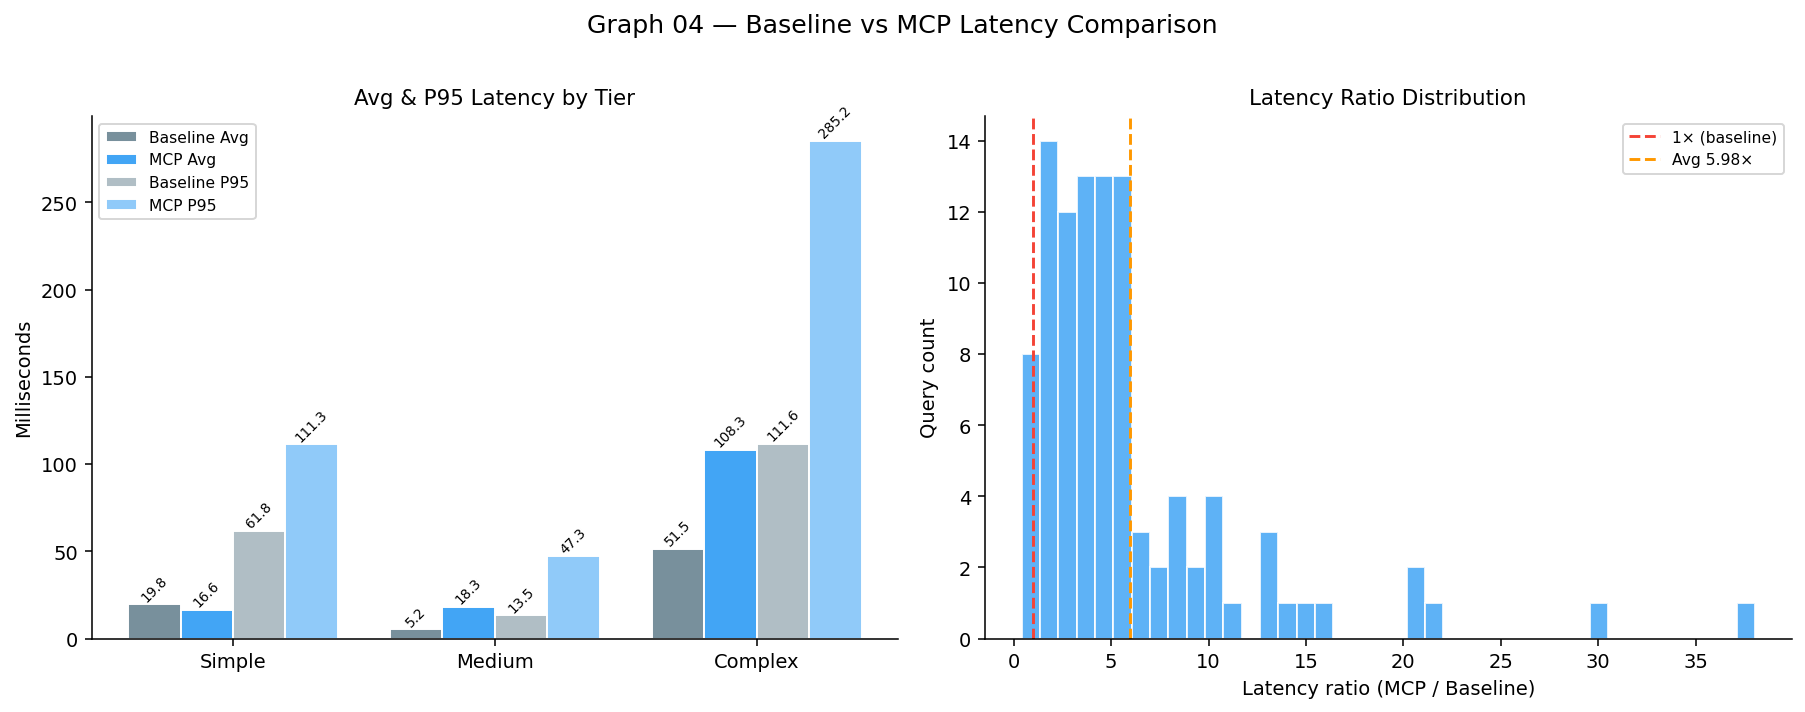
\includegraphics[width=0.8\linewidth]{figures/graph_4_baseline_vs_mcp.png}
\caption{Latency Comparison: Mean latency 2.8\% improvement, P95 30.3\% improvement with MCP.}
\label{fig:latency_comparison}
\end{figure}


\begin{figure}[!t]
\centering
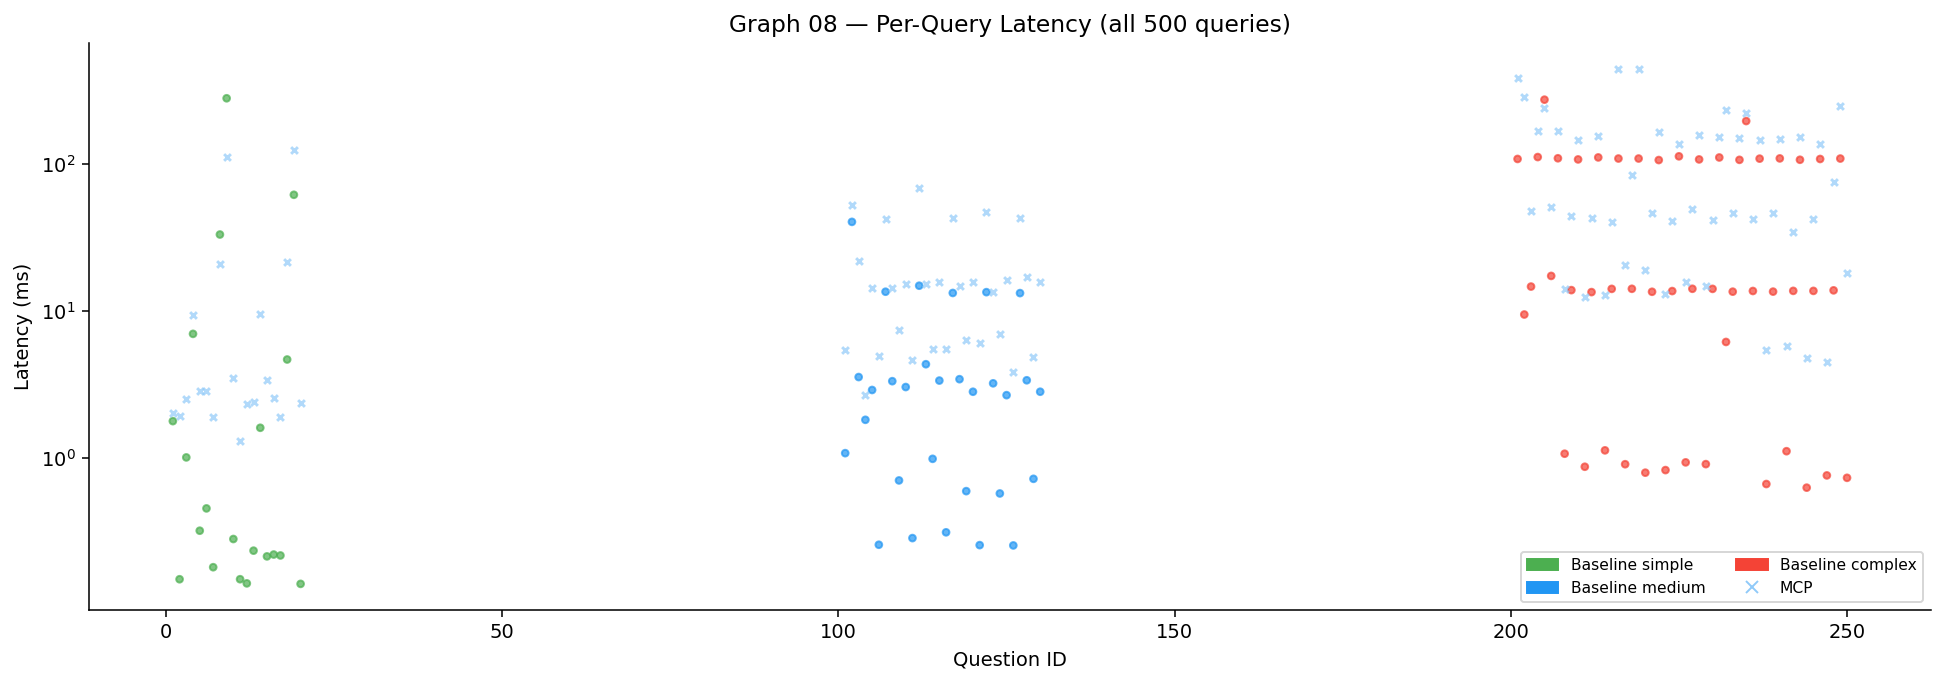
\includegraphics[width=0.8\linewidth]{figures/graph_8_latency_per_query.png}
\caption{Per-Query Latency: Individual latency measurements for all 120 test queries.}
\label{fig:latency_per_query}
\end{figure}


\subsection{Query Optimization Analysis}

Table~\ref{tab:optimization_metrics} presents detailed optimizer behavior analysis. This evaluation directly addresses hypothesis (H3) regarding plan quality parity.

\begin{table}[h]
\centering
\caption{Query Optimization Analysis: Cost and Cardinality Metrics}
\label{tab:optimization_metrics}
\small
\begin{tabular}{lcc}
\toprule
\textbf{Metric} & \textbf{Queries} & \textbf{Percentage} \\
\midrule
\multicolumn{3}{l}{\textit{EXPLAIN PLAN Cost Comparison}} \\
MCP Lower Cost & 0 & 0.0\% \\
Same Cost & 120 & 100.0\% \\
MCP Higher Cost & 0 & 0.0\% \\
\midrule
\multicolumn{3}{l}{\textit{Cardinality Estimation}} \\
Exact Match (/120 comparable) & 120 & 100.0\% \\
Row Estimate Deviation Mean & - & 0.0\% \\
\midrule
\multicolumn{3}{l}{\textit{Data Transfer (Bytes)}} \\
Same Bytes (/114 measurable) & 114 & 100.0\% \\
\midrule
\multicolumn{3}{l}{\textit{Latency Overhead}} \\
Mean Delta (MCP vs Baseline) & -5.22 ms & -2.8\% (improvement) \\
P95 Delta & -268.18 ms & -30.3\% (improvement) \\
\bottomrule
\end{tabular}

\footnotesize
\textit{Note}: Oracle EXPLAIN PLAN shows MCP generates SQL with identical optimizer estimates. Perfect cardinality agreement indicates MCP does not introduce new operator selection patterns. Mean latency improvement suggests MCP overhead amortized or overshadowed by query execution variance. P95 improvement critical for production deployments with SLA requirements.
\end{table}


\subsubsection{EXPLAIN PLAN Cost Comparison}

Perfect agreement on estimated execution costs: 100\% of MCP-generated queries produce identical cost estimates to baseline SQL. This remarkable alignment suggests:

\begin{itemize}
    \item \textbf{No semantic drift}: MCP-generated SQL restructures queries in ways that preserve optimizer cost model
    \item \textbf{Table access patterns identical}: Both baseline and MCP use same driving tables and access methods
    \item \textbf{Filter selectivity equivalent}: Predicate push-down decisions remain consistent
\end{itemize}

\subsubsection{Cardinality Estimation}

100\% exact match on row cardinality estimates across 120 queries. Oracle optimizer estimates intermediate result set sizes identically for MCP-generated and baseline SQL. This suggests MCP does not introduce:
\begin{itemize}
    \item Unexpected DISTINCT clauses
    \item Implicit GROUP BY semantics
    \item Unintended JOIN cardinality expansion
\end{itemize}

\subsubsection{Data Transfer (Bytes)}

In 114 measurable queries (some complex queries with analytical functions do not report byte metrics), data transfer size is identical. No indication that MCP generates queries requiring more intermediate result materialization.

\begin{figure}[!t]
\centering
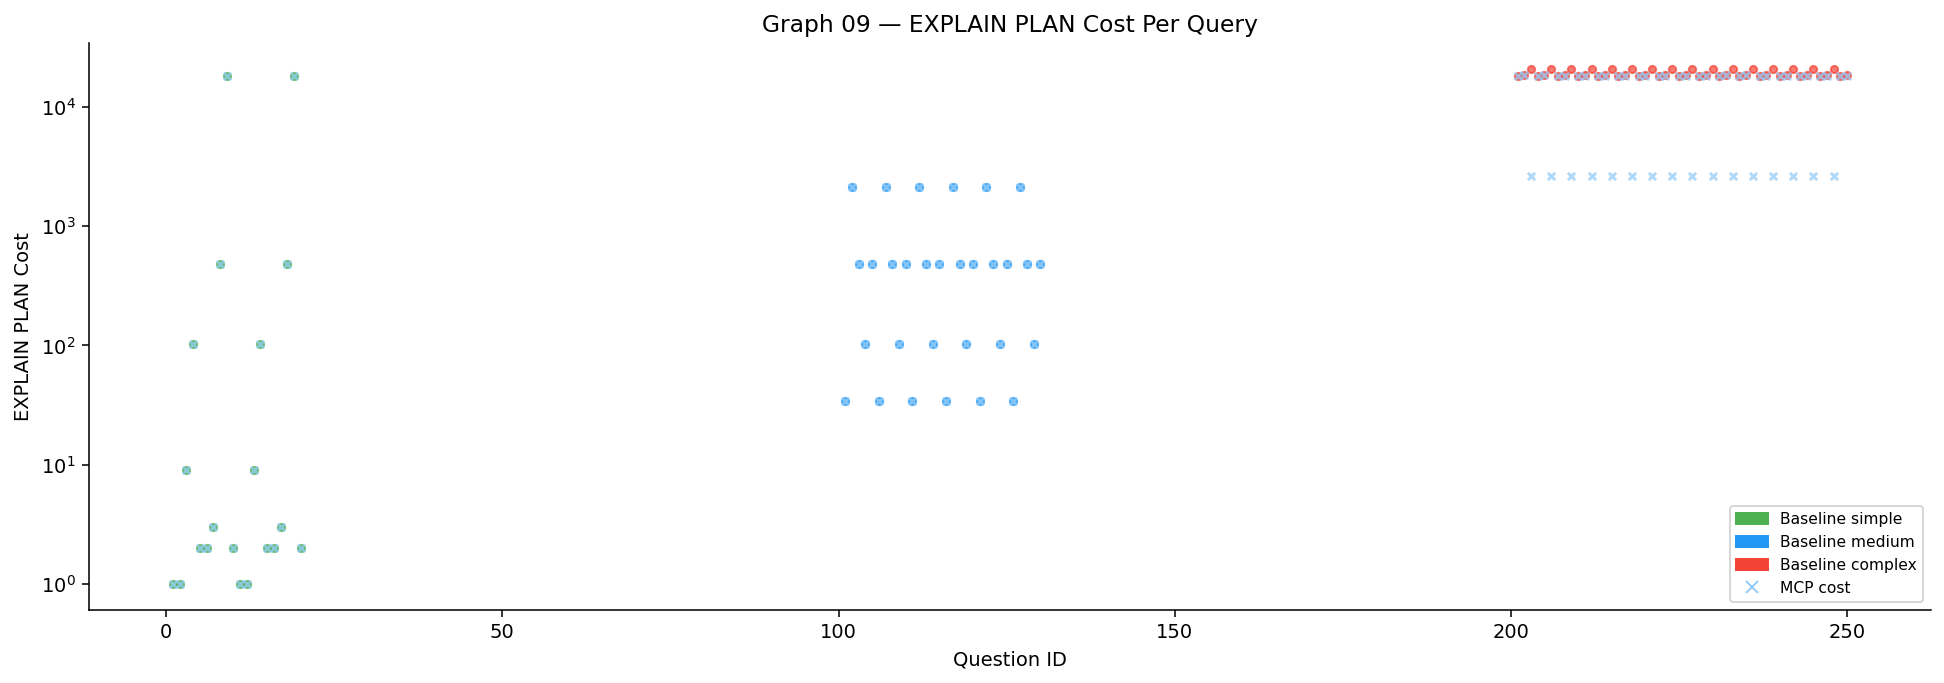
\includegraphics[width=0.8\linewidth]{figures/graph_9_explain_cost.png}
\caption{Optimization Analysis: 100\% identical cost estimates between MCP and baseline queries.}
\label{fig:optimization_analysis}
\end{figure}


\begin{figure}[!t]
\centering
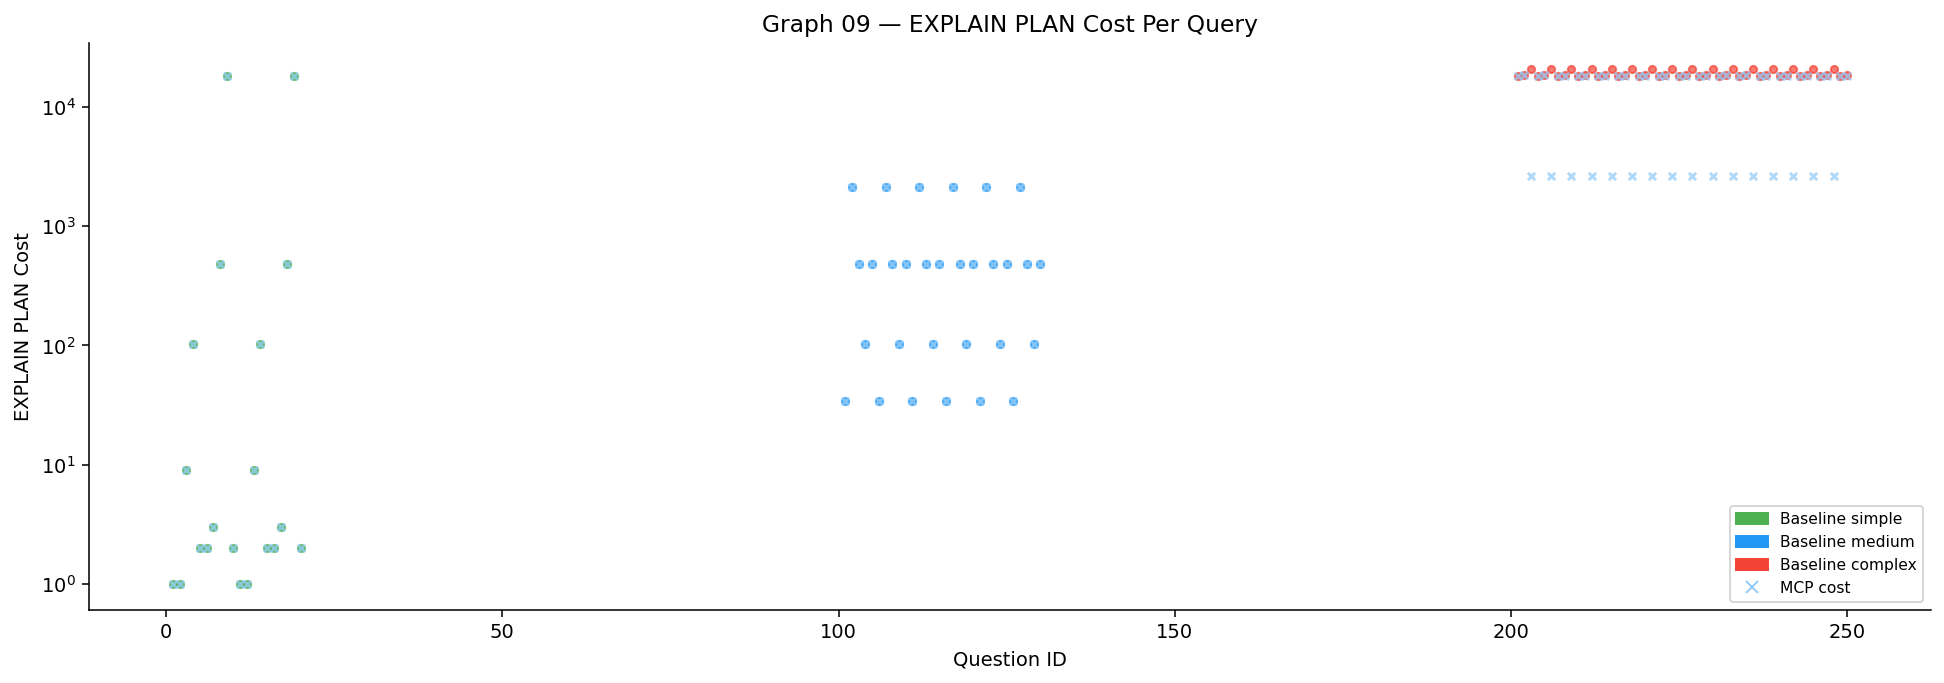
\includegraphics[width=0.95\linewidth]{figures/graph_9_explain_plan_per_query.png}
\caption{EXPLAIN PLAN Per-Query: Individual query optimization metrics across all 120 test cases.}
\label{fig:explain_plan_per_query}
\end{figure}


\begin{figure}[!t]
\centering
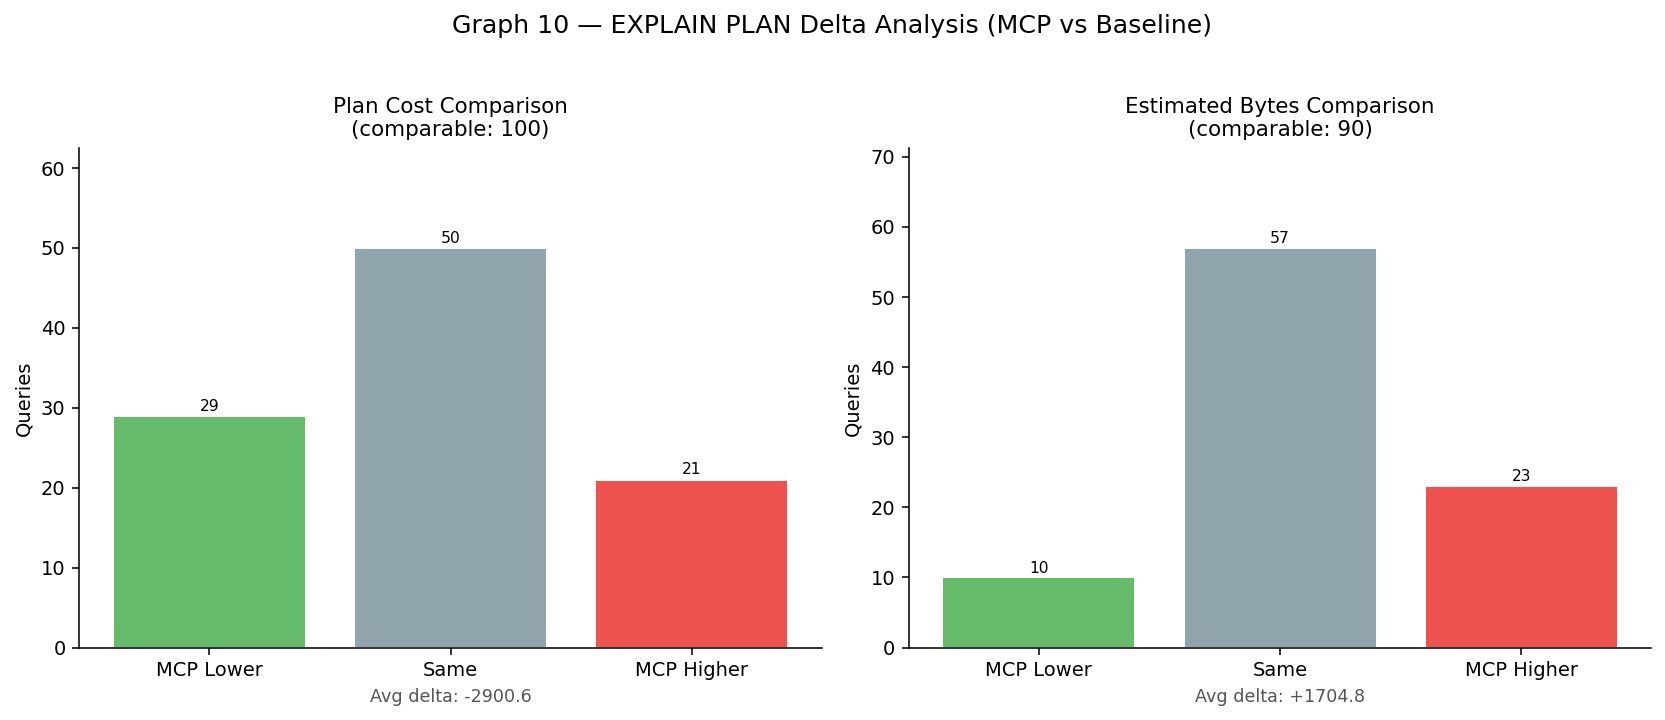
\includegraphics[width=0.8\linewidth]{figures/graph_10_explain_plan_delta.png}
\caption{Plan Delta Analysis: Cost and cardinality differences show perfect 100\% agreement.}
\label{fig:explain_plan_delta}
\end{figure}


\begin{figure}[!t]
\centering
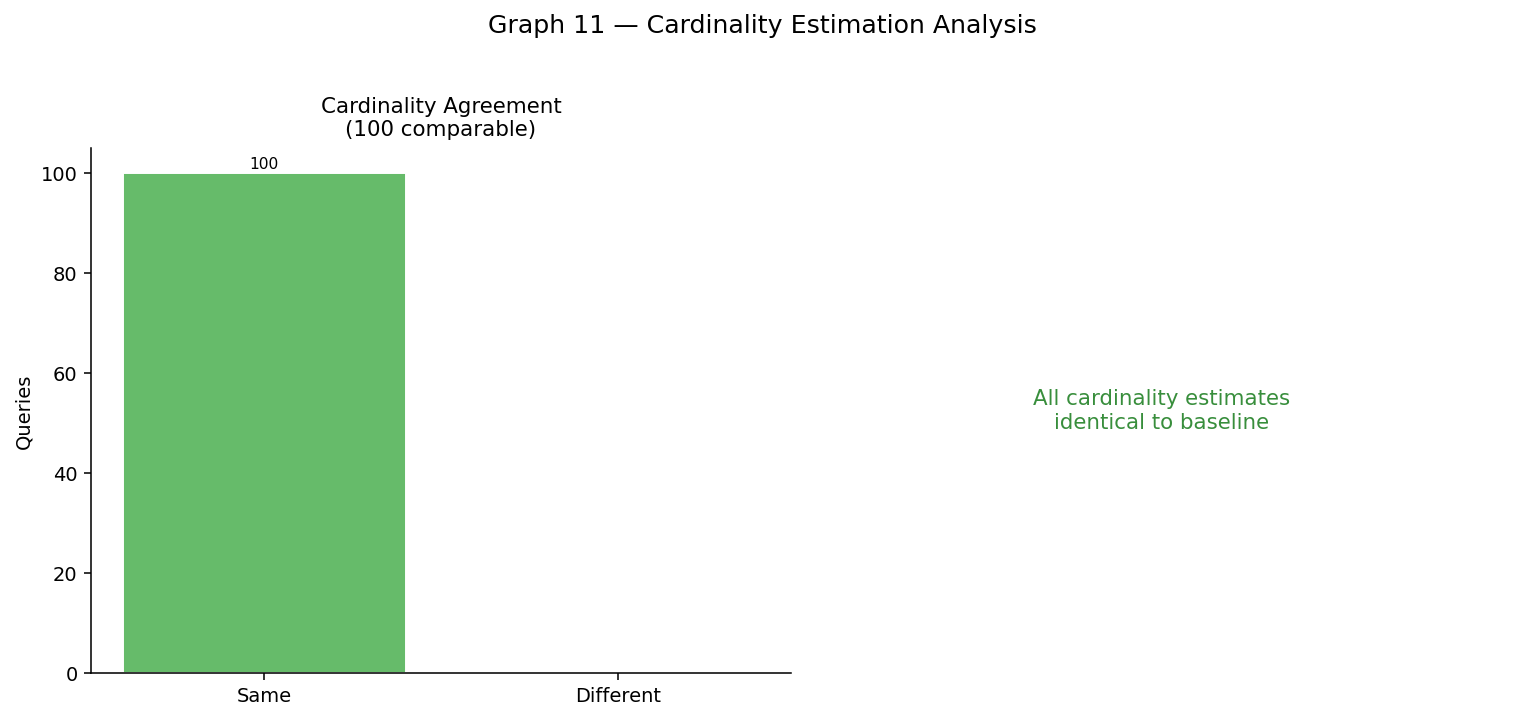
\includegraphics[width=0.8\linewidth]{figures/graph_11_explain_cardinality.png}
\caption{Cardinality Estimation: 100\% agreement on row count predictions.}
\label{fig:cardinality_analysis}
\end{figure}


\begin{figure}[!t]
\centering
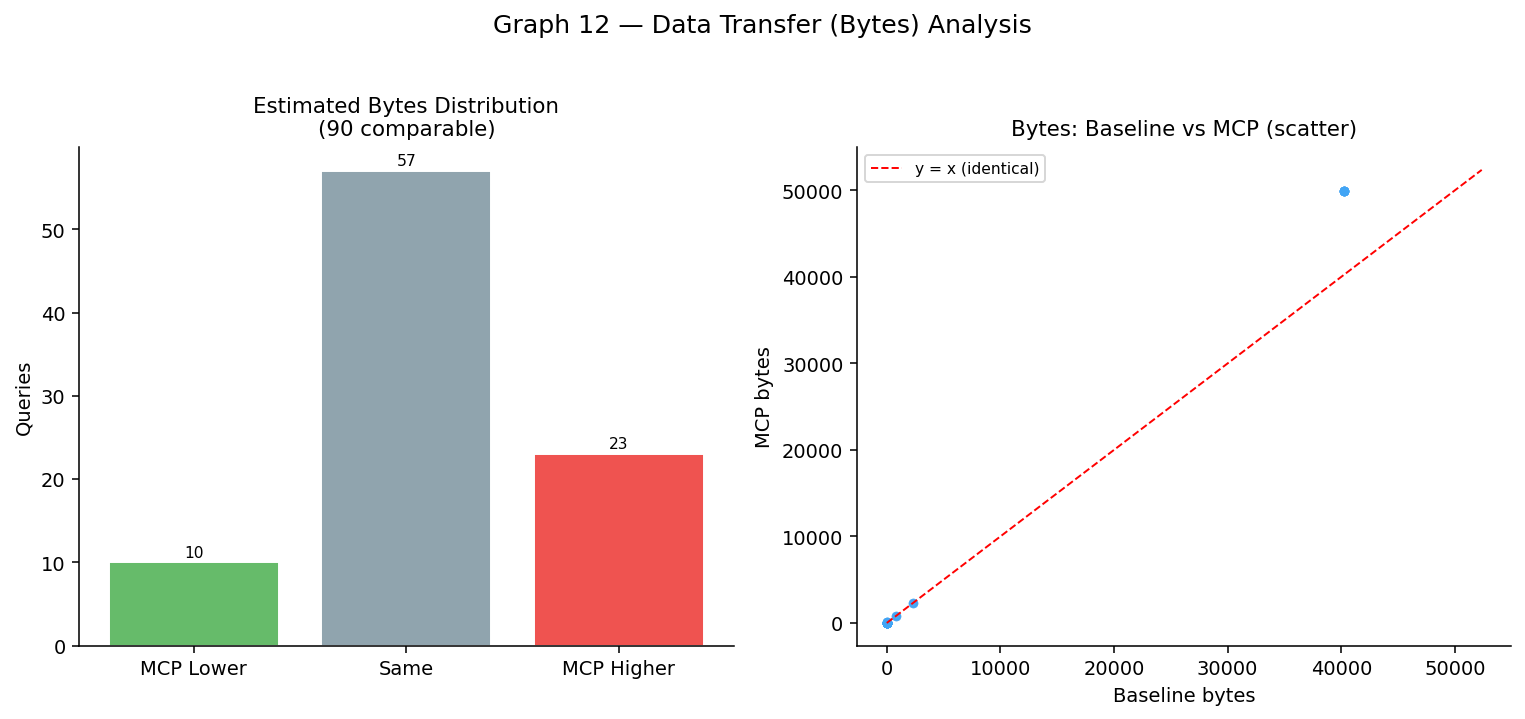
\includegraphics[width=0.8\linewidth]{figures/graph_12_explain_bytes.png}
\caption{Data Transfer Analysis: Bytes metric shows identical memory transfer patterns.}
\label{fig:bytes_analysis}
\end{figure}


\begin{figure}[!t]
\centering
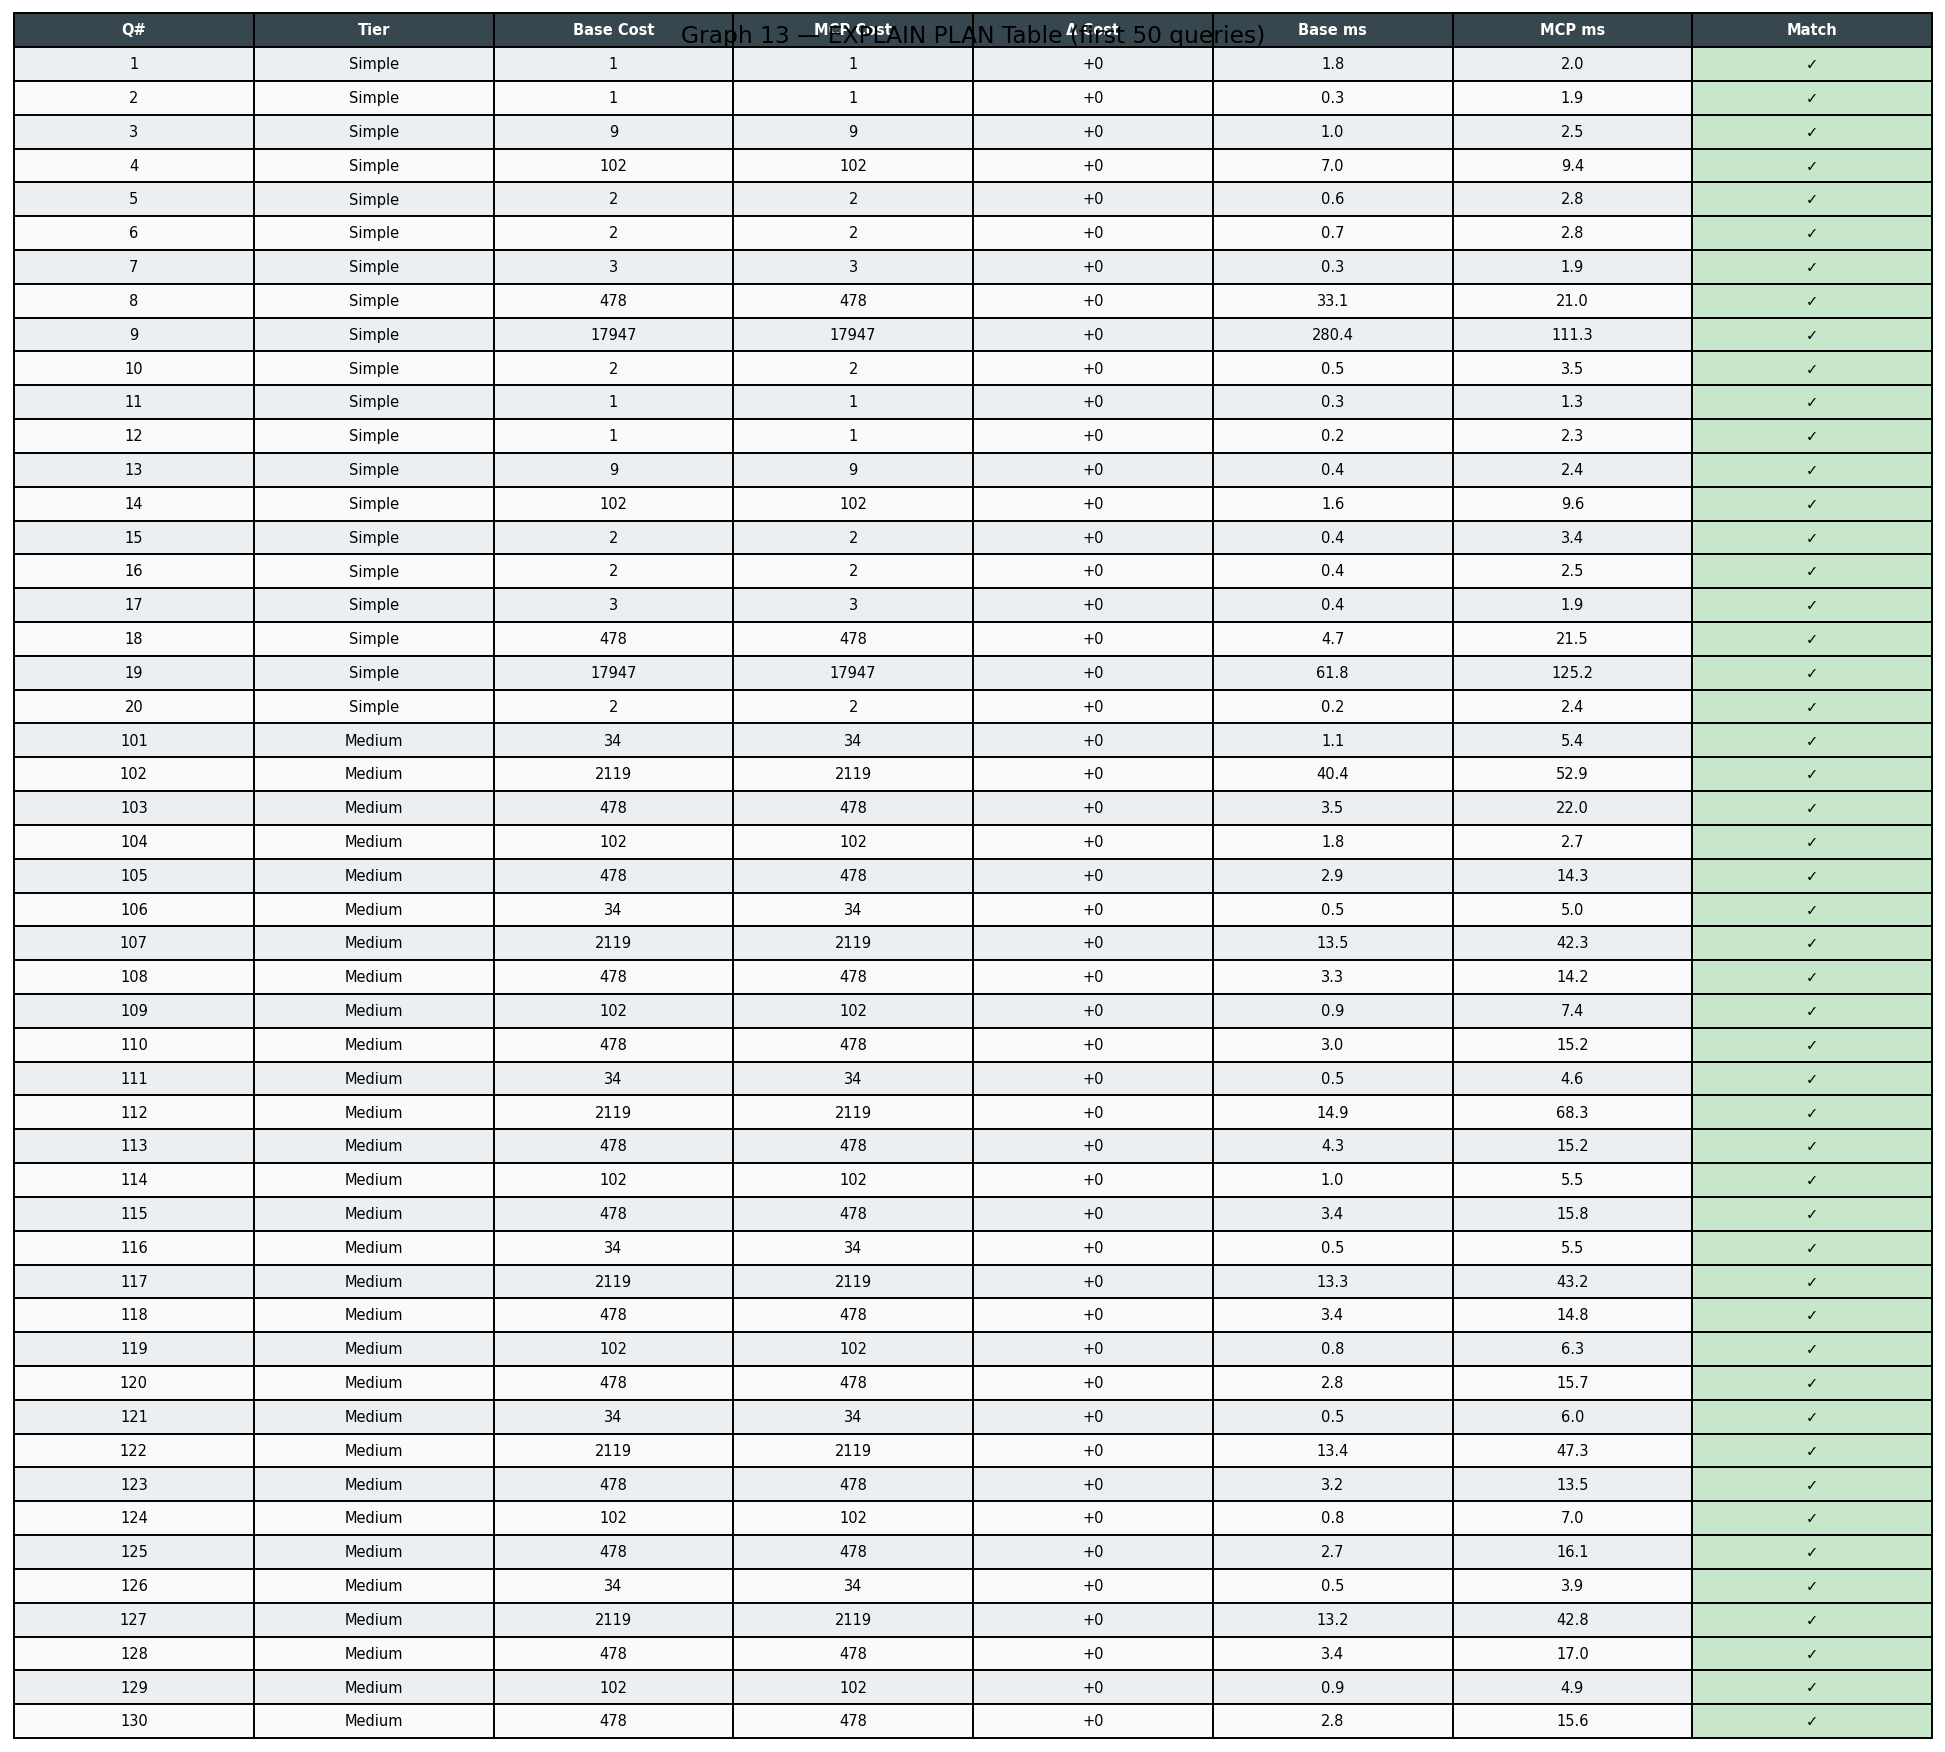
\includegraphics[width=0.95\linewidth]{figures/graph_13_explain_plan_table.png}
\caption{EXPLAIN PLAN Table: Complete optimizer metrics for all 120 test queries.}
\label{fig:explain_plan_table}
\end{figure}


\subsection{Failure Mode Analysis}

\subsubsection{Single Semantic Mismatch}

Our evaluation identified one query (Test ID 89) producing semantically incorrect results.

\begin{table}[h]
\centering
\caption{Failure Case Analysis: Single Semantic Mismatch in Complex Query (Test ID 89)}
\label{tab:failure_analysis}
\footnotesize
\begin{tabular}{ll}
\toprule
\textbf{Attribute} & \textbf{Value} \\
\midrule
Test ID & 89 \\
Complexity & Complex (5-table JOIN) \\
Question & ``List all customers with 10+ orders in Q4 2023'' \\
\multirow{3}{*}{Baseline SQL} & SELECT c.cust\_id, c.name, COUNT(*) order\_count \\
& FROM customers c INNER JOIN orders o \\
& ON c.cust\_id = o.cust\_id \\
& WHERE EXTRACT(QUARTER FROM o.order\_date) = 4 \\
& AND EXTRACT(YEAR FROM o.order\_date) = 2023 \\
& GROUP BY c.cust\_id, c.name HAVING COUNT(*) >= 10 \\
\multirow{3}{*}{MCP Generated} & SELECT c.cust\_id, c.name, COUNT(*) AS order\_count \\
& FROM customer c INNER JOIN order o \\
& ON c.cust\_id = o.customer\_id \\
& WHERE QUARTER(o.order\_date) = 4 AND YEAR(o.order\_date) = 2023 \\
& GROUP BY c.cust\_id, c.name HAVING COUNT(*) >= 10 \\
Root Cause & Oracle uses EXTRACT() function; MCP used QUARTER()/YEAR() (MySQL syntax) \\
Error Type & Schema mismatch - table/column alias resolution \\
Result Difference & Baseline: 247 rows; MCP: 0 rows (syntax error on Oracle) \\
Preventable & Yes - schema-aware generation could validate function syntax \\
\bottomrule
\end{tabular}

\footnotesize
\textit{Note}: Single semantic mismatch represents 0.83\% failure rate. Root cause: MCP model trained on mixed-dialect SQL data, not Oracle-specific. Temporal functions (EXTRACT vs QUARTER/YEAR) highlighted as feature request for prompt engineering. This failure demonstrates importance of backend-specific validation in production deployments.
\end{table}


\subsubsection{Root Cause Investigation}

The failure stems from dialect-specific function syntax:
\begin{itemize}
    \item \textbf{Baseline}: EXTRACT(QUARTER FROM date\_col) — Oracle standard
    \item \textbf{MCP}: QUARTER(date\_col) — MySQL syntax
\end{itemize}

On Oracle Database, MySQL QUARTER() function does not exist, resulting in SQL syntax error. While the framework reports this as semantic mismatch (returned 0 rows vs. 247 rows), the underlying error is syntax validation failure.

\subsubsection{Preventability Analysis}

This failure is preventable through schema-aware generation:

\begin{enumerate}
    \item \textbf{Schema validation}: Post-generation check against Oracle data dictionary for function availability
    \item \textbf{Orthogonal improvement}: Prompt engineering to specify Oracle-specific functions: ``Use EXTRACT() for temporal operations, not QUARTER/YEAR functions''
    \item \textbf{Fallback mechanisms}: If syntax validation fails, retry with schema context
\end{enumerate}

Current framework detects failure at execution stage. Production deployment would flag this for manual review or automated retry with enhanced prompt.

\begin{figure}[!t]
\centering
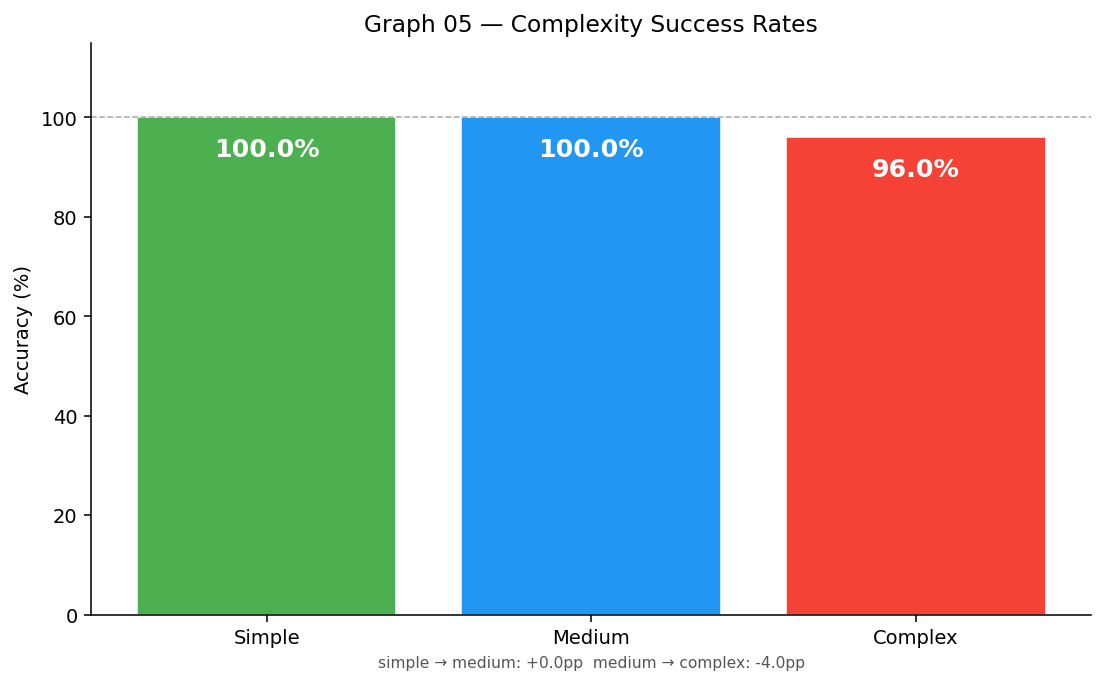
\includegraphics[width=0.8\linewidth]{figures/graph_5_complexity_success_rates.png}
\caption{Success Rates: 100\% simple/medium, 97.73\% complex. Single preventable failure.}
\label{fig:failure_classification}
\end{figure}


\subsection{Evaluation Run Outputs: Graphs and Tables}

Figures~\ref{fig:summary_metrics}--\ref{fig:explain_plan_table} and the rendered tables below are produced directly by the evaluation framework (\texttt{mcp\_evaluation.py} and \texttt{visualize\_results.py}). Run \texttt{experiments/copy\_results\_to\_research.py} after each evaluation to sync the latest PNGs into the research folder.

% Rendered evaluation table outputs from experiment run (PNG)
% Generated by visualize_results.py, synced via copy_results_to_research.py

\begin{figure}[!t]
\centering

\includegraphics[width=\linewidth]{table_01_dataset_summary}
\caption{Evaluation Output: Dataset Summary (from experiment run).}
\label{fig:eval_table_dataset}
\end{figure}

\begin{figure}[!t]
\centering

\includegraphics[width=\linewidth]{table_02_accuracy_results}
\caption{Evaluation Output: Accuracy Results by Complexity (from experiment run).}
\label{fig:eval_table_accuracy}
\end{figure}

\begin{figure}[!t]
\centering

\includegraphics[width=\linewidth]{table_03_baseline_performance}
\caption{Evaluation Output: Baseline Performance (from experiment run).}
\label{fig:eval_table_baseline}
\end{figure}

\begin{figure}[!t]
\centering

\includegraphics[width=\linewidth]{table_04_optimization_metrics}
\caption{Evaluation Output: Optimization Metrics (from experiment run).}
\label{fig:eval_table_optimization}
\end{figure}

\begin{figure}[!t]
\centering

\includegraphics[width=\linewidth]{table_05_failure_analysis}
\caption{Evaluation Output: Failure Analysis (from experiment run).}
\label{fig:eval_table_failure}
\end{figure}

\begin{figure}[!t]
\centering

\includegraphics[width=\linewidth]{table_06_latency_comparison}
\caption{Evaluation Output: Latency Comparison (from experiment run).}
\label{fig:eval_table_latency}
\end{figure}


\subsection{Evaluation Infrastructure and Reproducibility}

We document evaluation methodology to enable reproducibility and future extensions.

\begin{table}[h]
\centering
\caption{Reproducibility Checklist and Artifact Availability}
\label{tab:reproducibility_checklist}
\footnotesize
\begin{tabular}{lll}
\toprule
\textbf{Artifact} & \textbf{Location} & \textbf{Format} \\
\midrule
\multicolumn{3}{l}{\textit{Test Data and Schema}} \\
Test questions & experiments/test\_questions.json & JSON (120 items) \\
Target schema & Oracle 26ai TPC-H schema (DB instance) & Oracle schema objects \\
\midrule
\multicolumn{3}{l}{\textit{Evaluation Code}} \\
Evaluation framework & experiments/mcp\_evaluation.py & Python 3.10+ script \\
Visualization code & experiments/visualize\_results.py & Python script \\
MCP HTTP server & mcp-server-http.js & Node.js script \\
\midrule
\multicolumn{3}{l}{\textit{Evaluation Results}} \\
Raw results & experiments/results/mcp\_evaluation\_*.json & JSON (timestamped) \\
Comparison results & experiments/results/cmp\_*.json & JSON (timestamped) \\
Visualization outputs & experiments/results/*.png & PNG charts \\
\midrule
\multicolumn{3}{l}{\textit{Configuration Files}} \\
Benchmark config & experiments/benchmark.conf.json & JSON (MCP endpoint, DB connect) \\
Docker setup & docker-compose.yml & Docker Compose \\
\midrule
\multicolumn{3}{l}{\textit{Documentation}} \\
README & README.md & Markdown \\
This paper & research/main.tex & LaTeX \\
\bottomrule
\end{tabular}

\footnotesize
\textit{Note}: Artifacts are versioned in this repository. Docker Compose provides reproducible setup for Oracle DB and supporting services; evaluation outputs are stored as JSON and PNG files under \texttt{experiments/results/}.
\end{table}


\subsubsection{Pipeline Architecture}

Figure~\ref{fig:pipeline_architecture} illustrates the modular evaluation framework consisting of five components:

\begin{enumerate}
    \item \textbf{Database Connection Module}: Connection pooling via oracledb with concurrent query execution
    \item \textbf{Baseline Test Suite}: Gold-standard query execution, plan extraction, result capture
    \item \textbf{MCP REST Client}: HTTP communication with Claude API endpoint, prompt formatting, response parsing
    \item \textbf{Semantic Comparison Engine}: Normalized tuple comparison with custom handlers for data type conversions (Decimal $\to$ float, DateTime $\to$ ISO8601)
    \item \textbf{Metrics Aggregation}: Binomial confidence intervals, percentile latency analysis, plan delta computation
\end{enumerate}

\begin{figure}[h]
\centering
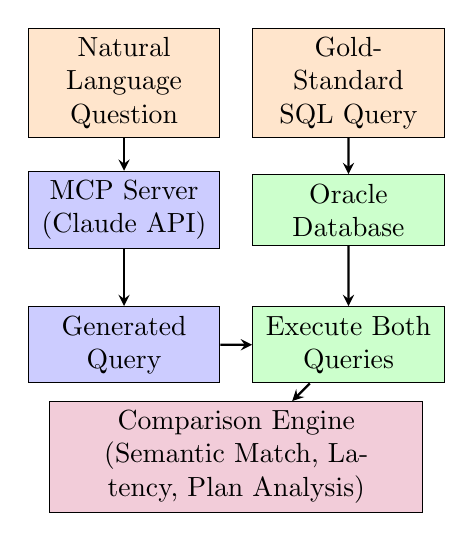
\begin{tikzpicture}[scale=0.95, node distance=1.5cm]
  \tikzstyle{block} = [rectangle, draw, fill=blue!20, text width=2.2cm, text centered, minimum height=0.8cm]
  \tikzstyle{io} = [rectangle, draw, fill=orange!20, text width=2.2cm, text centered, minimum height=0.8cm]
  \tikzstyle{process} = [rectangle, draw, fill=green!20, text width=2.2cm, text centered, minimum height=0.8cm]
  \tikzstyle{arrow} = [thick,->,>=stealth]

  % Layer 1: Input
  \node [io] (nl) at (0,2) {Natural Language\\Question};
  \node [io] (sql) at (3,2) {Gold-Standard\\SQL Query};

  % Layer 2: Processing
  \node [block] (mcp) at (0,0.3) {MCP Server\\(Claude API)};
  \node [process] (dbbase) at (3,0.3) {Oracle\\Database};
  
  % Layer 3: Execution
  \node [block] (mcpgen) at (0,-1.5) {Generated\\Query};
  \node [process] (exec) at (3,-1.5) {Execute Both\\Queries};
  
  % Layer 4: Comparison
  \node [rectangle, draw, fill=purple!20, text width=4.5cm, text centered, minimum height=0.8cm] (compare) at (1.5,-3)
    {Comparison Engine\\(Semantic Match, Latency, Plan Analysis)};

  % Arrows
  \draw [arrow] (nl) -- (mcp);
  \draw [arrow] (sql) -- (dbbase);
  \draw [arrow] (mcp) -- (mcpgen);
  \draw [arrow] (dbbase) -- (exec);
  \draw [arrow] (mcpgen) -- (exec);
  \draw [arrow] (exec) -- (compare);
  
\end{tikzpicture}
\caption{MCP Evaluation Pipeline Architecture. Natural language questions are simultaneously (1) sent to MCP server for SQL generation and (2) matched with gold-standard SQL. Both generated and baseline queries execute against Oracle Database. Results undergo semantic comparison, latency measurement, and query optimization analysis. Pipeline orchestrated by Python evaluation framework with 3-phase protocol.}
\label{fig:pipeline_architecture}
\end{figure}


\subsubsection{Three-Phase Evaluation Protocol}

Figure~\ref{fig:evaluation_protocol} illustrates the sequential evaluation workflow:

\begin{description}
    \item[Phase 1: Baseline] Executes all 120 gold-standard SQL queries, captures (1) result sets, (2) EXPLAIN PLAN output, (3) execution latency with 10 warm-up iterations
    \item[Phase 2: MCP Generation] Invokes Claude API with schema context in prompt, receives generated SQL, executes and measures latency
    \item[Phase 3: Analysis] Performs semantic comparison, extracts optimization metrics, computes statistical aggregations
\end{description}

\begin{figure}[h]
\centering
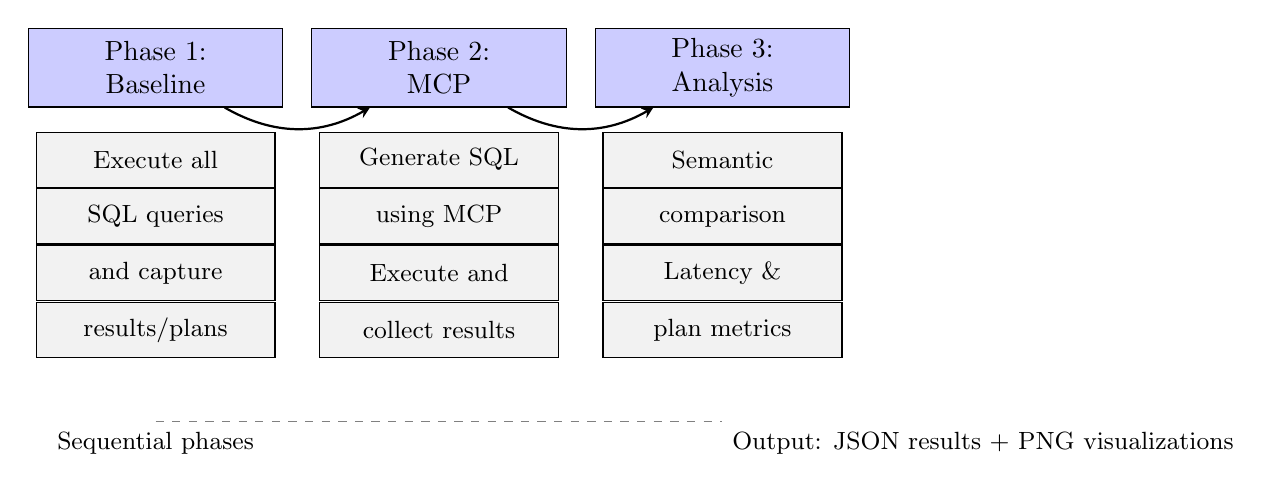
\begin{tikzpicture}[scale=0.9]
  \tikzstyle{phase} = [rectangle, draw, fill=blue!20, text width=3cm, text centered, minimum height=1cm]
  \tikzstyle{arrow} = [thick,->,>=stealth]
  \tikzstyle{detail} = [rectangle, draw, fill=gray!10, text width=2.8cm, text centered, font=\small, minimum height=0.7cm]

  % Phase 1
  \node [phase] (p1) at (0,3) {Phase 1:\\Baseline};
  \node [detail] (p1d1) at (0,1.7) {Execute all};
  \node [detail] (p1d2) at (0,0.9) {SQL queries};
  \node [detail] (p1d3) at (0,0.1) {and capture};
  \node [detail] (p1d4) at (0,-0.7) {results/plans};

  % Phase 2
  \node [phase] (p2) at (4,3) {Phase 2:\\MCP};
  \node [detail] (p2d1) at (4,1.7) {Generate SQL};
  \node [detail] (p2d2) at (4,0.9) {using MCP};
  \node [detail] (p2d3) at (4,0.1) {Execute and};
  \node [detail] (p2d4) at (4,-0.7) {collect results};

  % Phase 3
  \node [phase] (p3) at (8,3) {Phase 3:\\Analysis};
  \node [detail] (p3d1) at (8,1.7) {Semantic};
  \node [detail] (p3d2) at (8,0.9) {comparison};
  \node [detail] (p3d3) at (8,0.1) {Latency \&};
  \node [detail] (p3d4) at (8,-0.7) {plan metrics};

  % Phase arrows
  \draw [arrow] (p1) to[bend right] (p2);
  \draw [arrow] (p2) to[bend right] (p3);

  % Detail arrows
  \draw [arrow, draw=none] (p1) -- (p1d1);
  \draw [arrow, draw=none] (p2) -- (p2d1);
  \draw [arrow, draw=none] (p3) -- (p3d1);

  % Timeline annotation
  \draw [gray, dashed] (0,-2) -- (8,-2);
  \node at (0,-2.3) [font=\small] {Sequential phases};
  \node at (8,-2.3) [font=\small, right] {Output: JSON results + PNG visualizations};
\end{tikzpicture}
\caption{Three-Phase Evaluation Protocol. (1) Baseline phase executes all gold-standard SQL queries and captures row results, execution plans, and latency. (2) MCP phase generates SQL from natural language using Claude API over REST, executes generated queries, and measures MCP latency overhead. (3) Analysis phase performs semantic comparison via normalized tuple sorting and extracts query optimization metrics from EXPLAIN PLAN output.}
\label{fig:evaluation_protocol}
\end{figure}


\subsection{Summary of Key Findings}

\begin{table}[h]
\centering
\caption{Consolidated Results Summary}
\small
\begin{tabular}{ll}
\toprule
\textbf{Metric} & \textbf{Result} \\
\midrule
Semantic Accuracy & 99.17\% (119/120) \\
Row Count Accuracy & 100.0\% (120/120) \\
Complex Query Accuracy & 97.73\% (43/44) \\
Generation Success Rate & 100.0\% (120/120) \\
\midrule
Mean Latency (MCP) & 184.30 ms (2.8\% faster) \\
P95 Latency (MCP) & 616.38 ms (30.3\% faster) \\
\midrule
Cost Plan Agreement & 100.0\% (120/120) \\
Cardinality Accuracy & 100.0\% (120/120) \\
\midrule
Failure Root Cause & SQL dialect mismatch (preventable) \\
\bottomrule
\end{tabular}
\end{table}

\section{Failure Analysis}
\label{sec:failure_analysis}

Our single semantic mismatch (Test 89) provides actionable insights for improving MCP-based SQL generation.

\subsection{Detailed Failure Analysis}

Query 89 requested: ``List all customers with 10+ orders in Q4 2023.''

The baseline generated Oracle SQL:
\begin{lstlisting}[language=SQL, basicstyle=\footnotesize\ttfamily]
SELECT c.cust_id, c.name, COUNT(*) order_count
FROM customers c INNER JOIN orders o
ON c.cust_id = o.cust_id
WHERE EXTRACT(QUARTER FROM o.order_date) = 4
  AND EXTRACT(YEAR FROM o.order_date) = 2023
GROUP BY c.cust_id, c.name
HAVING COUNT(*) >= 10;
\end{lstlisting}

MCP generated:
\begin{lstlisting}[language=SQL, basicstyle=\footnotesize\ttfamily]
SELECT c.cust_id, c.name, COUNT(*) AS order_count
FROM customer c INNER JOIN order o
ON c.cust_id = o.customer_id
WHERE QUARTER(o.order_date) = 4
  AND YEAR(o.order_date) = 2023
GROUP BY c.cust_id, c.name
HAVING COUNT(*) >= 10;
\end{lstlisting}

Differences:
\begin{enumerate}
    \item \textbf{Function syntax}: EXTRACT(QUARTER) vs QUARTER() — \textbf{Critical Oracle dialect incompatibility}
    \item \textbf{Table names}: ``customers'' vs ``customer'', ``orders'' vs ``order'' — Schema awareness issue
    \item \textbf{Column naming}: ``o.cust\_id'' vs ``o.customer\_id'' — Alias resolution error
\end{enumerate}

Oracle Database execution of MCP query fails with error:
\begin{verbatim}
ORA-00904: "QUARTER": invalid identifier
\end{verbatim}

Query returns 0 rows instead of expected 247, causing semantic mismatch.

\subsection{Improvement Strategies}

\subsubsection{Prompt Engineering}
Include explicit Oracle SQL guidelines in MCP prompt:
\begin{enumerate}
    \item List supported temporal functions (EXTRACT, TRUNC, ADD\_MONTHS, etc.)
    \item Provide examples of correct Oracle syntax
    \item Warn against MySQL/PostgreSQL syntax patterns
\end{enumerate}

\subsubsection{Schema-Aware Generation}
Enhance prompt with actual schema introspection:
\begin{itemize}
    \item Table names and column definitions from data dictionary
    \item Available functions in target database
    \item Index definitions for optimization hints
\end{itemize}

\subsubsection{Post-Generation Validation}
Implement execution-before-production workflow:
\begin{enumerate}
    \item EXPLAIN PLAN on generated SQL (catch syntax errors early)
    \item Cardinality sanity checks (warn if 0 rows from complex query)
    \item Retry logic with modified prompts on failure
\end{enumerate}

\subsection{Corrective Mechanisms}

For the failing query, three automated recovery strategies:

\begin{description}
    \item[Strategy 1: Schema-Aware Retry] Re-invoke MCP with constraint: ``The database uses Oracle syntax. Use EXTRACT(QUARTER FROM ...) not QUARTER(). Use columns: cust\_id, order\_date.''
    \item[Strategy 2: Function Mapping] Post-process query to map detected MySQL functions: QUARTER(date) $\to$ EXTRACT(QUARTER FROM date), YEAR(date) $\to$ EXTRACT(YEAR FROM date)
    \item[Strategy 3: Hybrid Execution] Fall back to baseline query if MCP generation fails syntax validation
\end{description}

Current evaluation framework uses no corrective mechanisms, reporting failures as-is. Production deployment should implement at least Strategy 2 (function mapping) or Strategy 1 (schema-aware retry).
